\documentclass[main.tex]{subfiles}
\begin{document}
\label{sec:QASTest}
\section{Quality Attribute Scenario Tests}
% Describe how each QAS was tested (method)
% 
This section covers how the quality attribute scenario(QAS) has been tested. This includes the setup for the different tests as well as the results generated. 
The section will be split into subsections addressing each scenario.

\subsection{QAS Privacy}
\label{sec:PrivacyTest}
In order to test the privacy QAS from \smartref{subsec:PrivacyTacticandScenario}, a simple node-js server was created. 

The server is created in with two entry points. The first entry point serves a HTML-file containing a script. The script contained in the HTML-file got two tasks: (1) set a cookie client side and (2) send a POST request to the second endpoint of the server. The POST-request to the server contains the cookie just created. When the POST-request is received on the server the cookie(s) are logged in the terminal. After the cookie(s) have been logged, the data from the body is processed and sent back to the client. The response also contains a \(Set-Cookie\) header, which the client browser interprets and creates a second cookie. The flow for the test is described in \autoref{fig:QASPrivacyFlow}.

\begin{figure}[h]
    \centering
    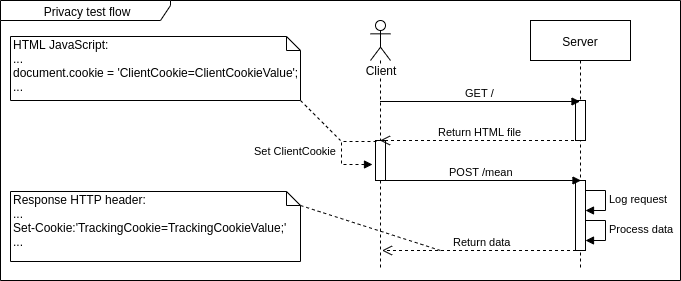
\includegraphics{Images/QAS-Test/QASPrivacyFlow.png}
    \caption{QAS privacy test flow}
    \label{fig:QASPrivacyFlow}
\end{figure}

The test was conducted by going through the flow described in \autoref{fig:QASPrivacyFlow} three times. The two first without YANF, and the last with YANF activated. The results from the server is shown in \autoref{lst:QAS-privacy-results}. The results show that first request contains the cookie set by the script in the HMTL-file. This is due to that the second cookie fist is set when the client get the response. The second time the request contains two requests as created by the first response. For the third request, YANF is activated. The results show that all cookies are removed from the request.


\begin{lstlisting}[
    language=sh,
    firstline=1, 
    frame=single, 
    caption={
        Cookie removal results
    },
    captionpos=b,
    label=lst:QAS-privacy-results
]
#YANF turned off:
1.st request
    Header:
        Cookies:
            - ClientCookie=ClientCookieValue

2.nd request
    Header:
        Cookies: 
            - ClientCookie=ClientCookieValue
            - TrackingCookie=TrackingCookieValue

#YANF turned on:
3.rd request
    Header:
        Cookies: 
\end{lstlisting}

YANF is made so that it removes the cookies from the request header. This is superior compared to removing the set-cookie header from the response. This is due to cookies are able to being set by JavaScript in the client it self. YANF is therefore both guarded against cookies being set by the response header and cookies being set by scripts. This functionality is show in \autoref{lst:QAS-privacy-results} by having let no cookies through. This fulfills the tactic specified in \autoref{subsec:PrivacyTacticandScenario}.


%The privacy scenario described in section \smartref{subsec:PrivacyTacticandScenario}, was run with both with and without YANF running on a mobile device. The setup for the test can be seen in \smartref{sec:PrivacyMethod}. The results shown in \autoref{lst:privacy}


\subsection{QAS Energy Efficiency}
\label{sec:EnergyTest}
The energy efficiency test has been created in order to verify if YANF comply with the response measure from the energy efficiency scenario described in \smartref{subsec:EnergyEfficiencyTacticandScenario}. The test consists of the following setup: the YANF application, a website with trackers and an android application loading the website and measuring the energy consumption of the phone. 

The goal of the test is to see the difference in energy consumption with YANF turned on vs. off. This is conducted over the duration of 1000 requests to \textit{cnet.com}. The reason \textit{cnet.com} was chosen for the test, was due to it being a known site making use of trackers. By utilizing the privacy browser \textit{Brave}, it is shown that 26 trackers is being blocked when loading the \textit{cnet.com} home page. 

In order to ensure the same conditions the phone is configured to the following specifications before starting the test each time:
\begin{itemize}
    \item Phone is a OnePlus 5
    \item Battery is 3300 mAh
    \item Battery is charged to 100\%
    \item All other applications than YANF and the test application is closed. 
    \item Internet is turned off for all other applications than YANF and the test application
    \item Screen brightness is set to 50\%
    \item Auto adjusting screen brightness is disabled
    \item Phone connected to WiFi
\end{itemize}

%charged fully before the test is started. Furthermore, the phone is stripped of all other applications using the internet connection. This is done so that the only thing using running on the phone and sending requests is YANF and the YANF-Energy-Test application. 

The energy test is run first with YANF turned off. This is done to have a base energy consumption. After the first test, the phone has been restored to the listed specifications. The test is then run again with YANF turned on. The results can be seen in \autoref{tab:energyConsumption1}.

\begin{table}[H]
    \centering
    \begin{tabular}{|l|l|}\hline
        \textbf{Test}   & \textbf{Power consumption}    \\ \hline
        YANF on         & 24\%                          \\ \hline
        YANF off        & 27\%                          \\ \hline
    \end{tabular}
    \caption{Energy consumption test for  loading \textit{cnet.com} 1000 times}
    \label{tab:energyConsumption1}
\end{table}

The results from the test shows that more power is consumed with YANF turned on. Furthermore, there is a very high power consumption for both tests. A hypothesis for this is the screen consuming the power. This might also affect the results of YANF being turned on, due to requests having a bit increased latency and therefore, the screen is turned on for a longer duration.

Based on the results a new test configuration was created. The new test is set up, so that the screen in turned off. This gives the following phone configuration for the second test:

\begin{itemize}
    \item Phone is a OnePlus 5
    \item Battery is 3300 mAh
    \item Battery is charged to 100\%
    \item All other applications than YANF and the test application is closed. 
    \item Internet is turned off for all other applications than YANF and the test application
    \item Phone connected to WiFi
    \item Screen is turned off for the duration of the test
\end{itemize}

The second test was run first with YANF off followed by it being on, resulting in the results seen in \autoref{tab:energyConsumption2}


\begin{table}[H]
    \centering
    \begin{tabular}{|l|l|}\hline
        \textbf{Test}   & \textbf{Power consumption}    \\ \hline
        YANF on         & 3\%                          \\ \hline
        YANF off        & 3\%                          \\ \hline
    \end{tabular}
    \caption{Second energy consumption test for loading \textit{cnet.com} 1000 times}
    \label{tab:energyConsumption2}
\end{table}

The results from the second test shows that screen was depleting the battery, and that YANF in it self does not deplete the battery. It should still be noted that by using YANF there will be a marginally increased latency and therefore increased screen time. Based on these results the hypothesis from \smartref{subsec:EnergyEfficiencyTacticandScenario} can not be rejected. Furthermore, YANF comply with the response measure specified for energy efficiency.

To further analyze the energy consumption of YANF, other tests should be done. An example of such tests could be to have a test group of users. These users could be monitored for a period without using YANF, followed up by a period of using it. This would give insight into how YANF  
\todoL{realistic use cases and further tests}
\todoL{Downsides to chosen test}

% Screen on
% YANF off - 1000 reqs - 24% power
% YANF on - 1000 reqs - 27% power


% Screen off
% YANF off - 1000 reqs - 3% power
% YANF on - 1000 reqs - 3% power

\end{document}